\documentclass[]{article}
\usepackage{lmodern}
\usepackage{amssymb,amsmath}
\usepackage{ifxetex,ifluatex}
\usepackage{fixltx2e} % provides \textsubscript
\ifnum 0\ifxetex 1\fi\ifluatex 1\fi=0 % if pdftex
  \usepackage[T1]{fontenc}
  \usepackage[utf8]{inputenc}
\else % if luatex or xelatex
  \ifxetex
    \usepackage{mathspec}
  \else
    \usepackage{fontspec}
  \fi
  \defaultfontfeatures{Ligatures=TeX,Scale=MatchLowercase}
\fi
% use upquote if available, for straight quotes in verbatim environments
\IfFileExists{upquote.sty}{\usepackage{upquote}}{}
% use microtype if available
\IfFileExists{microtype.sty}{%
\usepackage{microtype}
\UseMicrotypeSet[protrusion]{basicmath} % disable protrusion for tt fonts
}{}
\usepackage[margin=1in]{geometry}
\usepackage{hyperref}
\hypersetup{unicode=true,
            pdftitle={Harvard Data Science Capstone},
            pdfauthor={Tyson Klein},
            pdfborder={0 0 0},
            breaklinks=true}
\urlstyle{same}  % don't use monospace font for urls
\usepackage{graphicx,grffile}
\makeatletter
\def\maxwidth{\ifdim\Gin@nat@width>\linewidth\linewidth\else\Gin@nat@width\fi}
\def\maxheight{\ifdim\Gin@nat@height>\textheight\textheight\else\Gin@nat@height\fi}
\makeatother
% Scale images if necessary, so that they will not overflow the page
% margins by default, and it is still possible to overwrite the defaults
% using explicit options in \includegraphics[width, height, ...]{}
\setkeys{Gin}{width=\maxwidth,height=\maxheight,keepaspectratio}
\IfFileExists{parskip.sty}{%
\usepackage{parskip}
}{% else
\setlength{\parindent}{0pt}
\setlength{\parskip}{6pt plus 2pt minus 1pt}
}
\setlength{\emergencystretch}{3em}  % prevent overfull lines
\providecommand{\tightlist}{%
  \setlength{\itemsep}{0pt}\setlength{\parskip}{0pt}}
\setcounter{secnumdepth}{0}
% Redefines (sub)paragraphs to behave more like sections
\ifx\paragraph\undefined\else
\let\oldparagraph\paragraph
\renewcommand{\paragraph}[1]{\oldparagraph{#1}\mbox{}}
\fi
\ifx\subparagraph\undefined\else
\let\oldsubparagraph\subparagraph
\renewcommand{\subparagraph}[1]{\oldsubparagraph{#1}\mbox{}}
\fi

%%% Use protect on footnotes to avoid problems with footnotes in titles
\let\rmarkdownfootnote\footnote%
\def\footnote{\protect\rmarkdownfootnote}

%%% Change title format to be more compact
\usepackage{titling}

% Create subtitle command for use in maketitle
\newcommand{\subtitle}[1]{
  \posttitle{
    \begin{center}\large#1\end{center}
    }
}

\setlength{\droptitle}{-2em}

  \title{Harvard Data Science Capstone}
    \pretitle{\vspace{\droptitle}\centering\huge}
  \posttitle{\par}
    \author{Tyson Klein}
    \preauthor{\centering\large\emph}
  \postauthor{\par}
      \predate{\centering\large\emph}
  \postdate{\par}
    \date{October 22, 2018}


\begin{document}
\maketitle

\section{Analysis of RedBubble.com sales by
TysonK}\label{analysis-of-redbubble.com-sales-by-tysonk}

\subsection{An Overview}\label{an-overview}

RedBubble is one of the longest running and diverse Print-On-Demand
(POD) art websites in the world, offering artists everywhere a chance to
make money by selling their works on a range of products without having
to get involved with any of the logistics. As a homebody with a penchant
for Photoshop, I was naturally drawn to it.

Redbubble, like many of its contemporaries, has a `passive' approach for
the artist. You upload your designs as images, and they do everything
else. This means that all sales made are pure profit on the artists
side.

About a year and a half ago I opened
\href{https://www.redbubble.com/people/tysonk?ref=account-nav-dropdown\&asc=u}{my
Redbubble store}. The specifics of my store aren't entirely important to
this report, but there are some important details that will emerge again
later. Most designs I uploaded had something to do with National Parks
from English speaking countries around the world, and the remainder of
the designs are an eclectic mix of outdoors-themed and quirky pruducts
meant to appeal to a general audience.

The money started to come in, and as I tweaked some designs and
parameters within my store, I realized that this could be a legitimate
income stream. Beyond that, some interesting patterns began to emerge.
For example, although Redbubble offers designs to be printed on products
ranging from coffee mugs to T shirts to throw pillows, by far my most
sucessfull item was the sticker.

To date, stickers account for 98.5\% of all items sold and 96.2\% of all
revenue.

Below is the profit per day of my store since May 1st, 2017, measured in
Canadian Dollars.
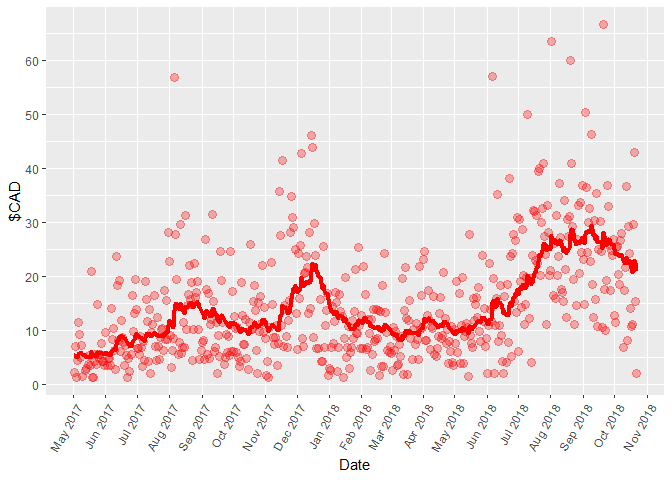
\includegraphics{Redbubble_Report_files/figure-latex/daily sales plot-1.pdf}

And here is the same graph for daily items sold.
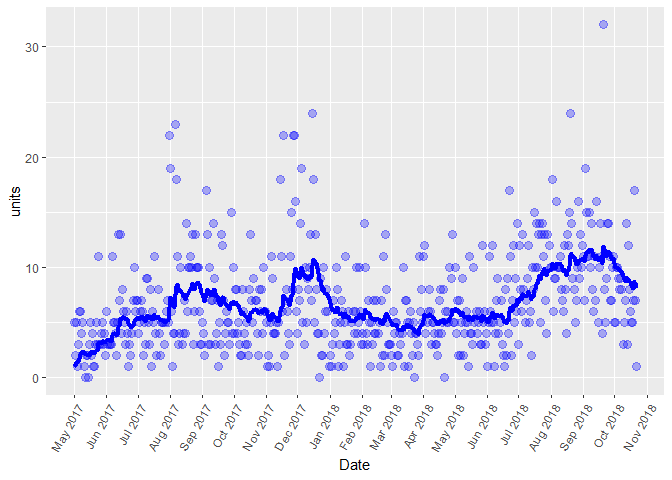
\includegraphics{Redbubble_Report_files/figure-latex/daily units plot-1.pdf}

As you can see by the similarity, each item sells for approximately the
same amount of money. This is mostly due to the volume of sticker sales
above other products, but the other interesting thing about these graphs
is the bump on the far right side of each graph. It is a bit hard to
tell, but the red bump rises a bit higher than the blue bump. This can
be summarized in the below graph, average dollars per item.

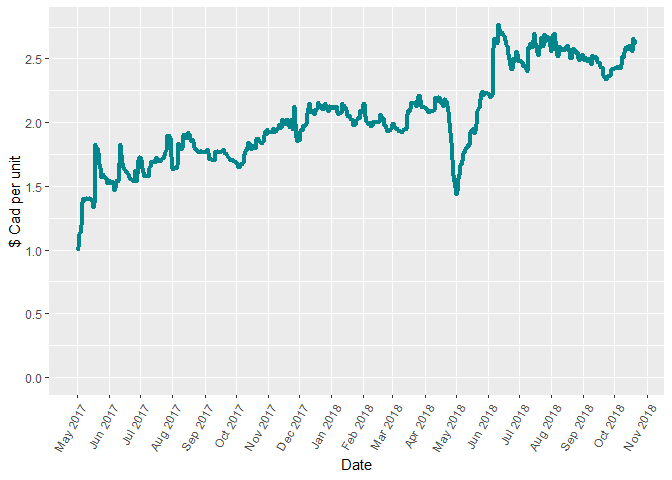
\includegraphics{Redbubble_Report_files/figure-latex/daily dollar per sale-1.pdf}

This is the result of a feature on Redbubble that has garnered a lot of
praise from artists on the platform. Artists are able to dictate
whatever profit margin they choose. These margins can be set product by
product, and even design by design, but the overwhelming majority of
people choose to leave this at the default setting of 20\%. This means
they make 20\% of the manufacturer cost, making each product cost 1.2X
the manufacturer cost.

\emph{This is a horrible idea.} The people at Redbubble are a group of
smart cookies and they know that the best way to sell more everything is
to make the artist margin as small as possible. My approach?
\textbf{crank it up to 11}

Within the first month of my time on Redbubble, I had my margin set to
90\%. My thoughts were that I could see how it changed the nature of my
sales data and find a happy middle ground nearer to their preset 20\%.
Not only did my profit go way up, but \emph{my daily units hardly
budged}. The chart above shows a few changes to this margin: Mid October
2017 up to 100\%, mid March 2018 up to 125\%, then an ill-advised change
down to 70\% in April shortly followed by a correction to 150\%, where
the margin has been ever since.

Those numbers might not seem to mean much, but for the average consumer
they certainly do. From the lowest point until now, the cost of a single
sticker in my shop has gone from about \$2.50 to \$6.00.


\end{document}
